

\section{Method}
\label{sec:methods}

%We first describe our classifier for detecting split errors which is based on a convolutional neural network (CNN). We detail the CNN architecture, input features and the training method. We then describe how the same classifier can be used to detect merge errors and how we create potential corrections. The classifiers are integrated into an existing proofreading workflow as reported after. Finally, we explore an active label suggestion method which reorders the ranking obtained by our classifiers and maximizes the information gain provided by each potential correction.
\subsection{Split Error Detection}

We build a split error classifier with output $p$ using a convolutional neural network (CNN) to check whether an edge within an existing automatic segmentation is valid ($p=0$) or not ($p=1$). Rather than analyzing every input pixel, the classifier operates only on segment boundaries which requires less pixel context and is faster. In contrast to Bogovic \etal~\cite{BogovicHJ13}, we work with 2D slices rather than 3D volumes. This enables proofreading prior or in parallel to an expensive alignment of individual EM images.
\\~\\
\textbf{Convolutional Neural Network Architecture.} Split error detection of a given boundary is really a binary classification task since the boundary is either correct or erroneous. However, in reality the score $p$ is between 0 and 1. The classification complexity arises from hundreds of different cell types in connectomics data rather than from the classification decision. Intuitively, this yields a wider (meaning more filters) rather than a deeper (meaning more layers) architecture. We explored different architectural configurations - including residual networks~\cite{resnet} - by performing a brute force parameter search and comparing precision and recall (see supplementary materials). Our final CNN configuration for split error detection is composed of four convolutional layers, each followed by max pooling as well as dropout regularization to prevent overfitting due to limited training data. Fig. \ref{fig:architecture} shows the CNN architecture for split error detection.
\\~\\
\textbf{Classifier Inputs.} To train the CNN for split error detection, we take boundary context information into consideration for the decision making process. For this, we use a $75\times75$ pixel patch at the center of an existing boundary. This covers approximately $80\%$ of all boundaries in real-world connectomics data with nanometer resolution. If the boundary edge is not fully covered, we sample up to 10 non-overlapping patches along the boundary and combine the resulting score by weighted averaging based on boundary length coverage per patch. 
Similar to Bogovich~\etal~\cite{BogovicHJ13}, we use grayscale image data, corresponding boundary probabilities, and a single binary mask combining the two neighboring labels as features for our CNN. However, we observed that the boundary probability information generated from EM images is often misleading due to noise or artifacts in the data. This can result in merge errors within the automatic segmentation. To better direct our classifier to train on the true boundary edge, we extract the border between two segments. We then dilate this border by 5 pixels to consider slight edge ambiguities and use this binary mask as an additional feature to create a stacked 4-channel input patch. Fig. \ref{fig:cnn_inputs} shows examples of correct and erroneous feature patches and their corresponding automatic segmentation and ground truth. 

\begin{figure}[h]
\begin{center}
  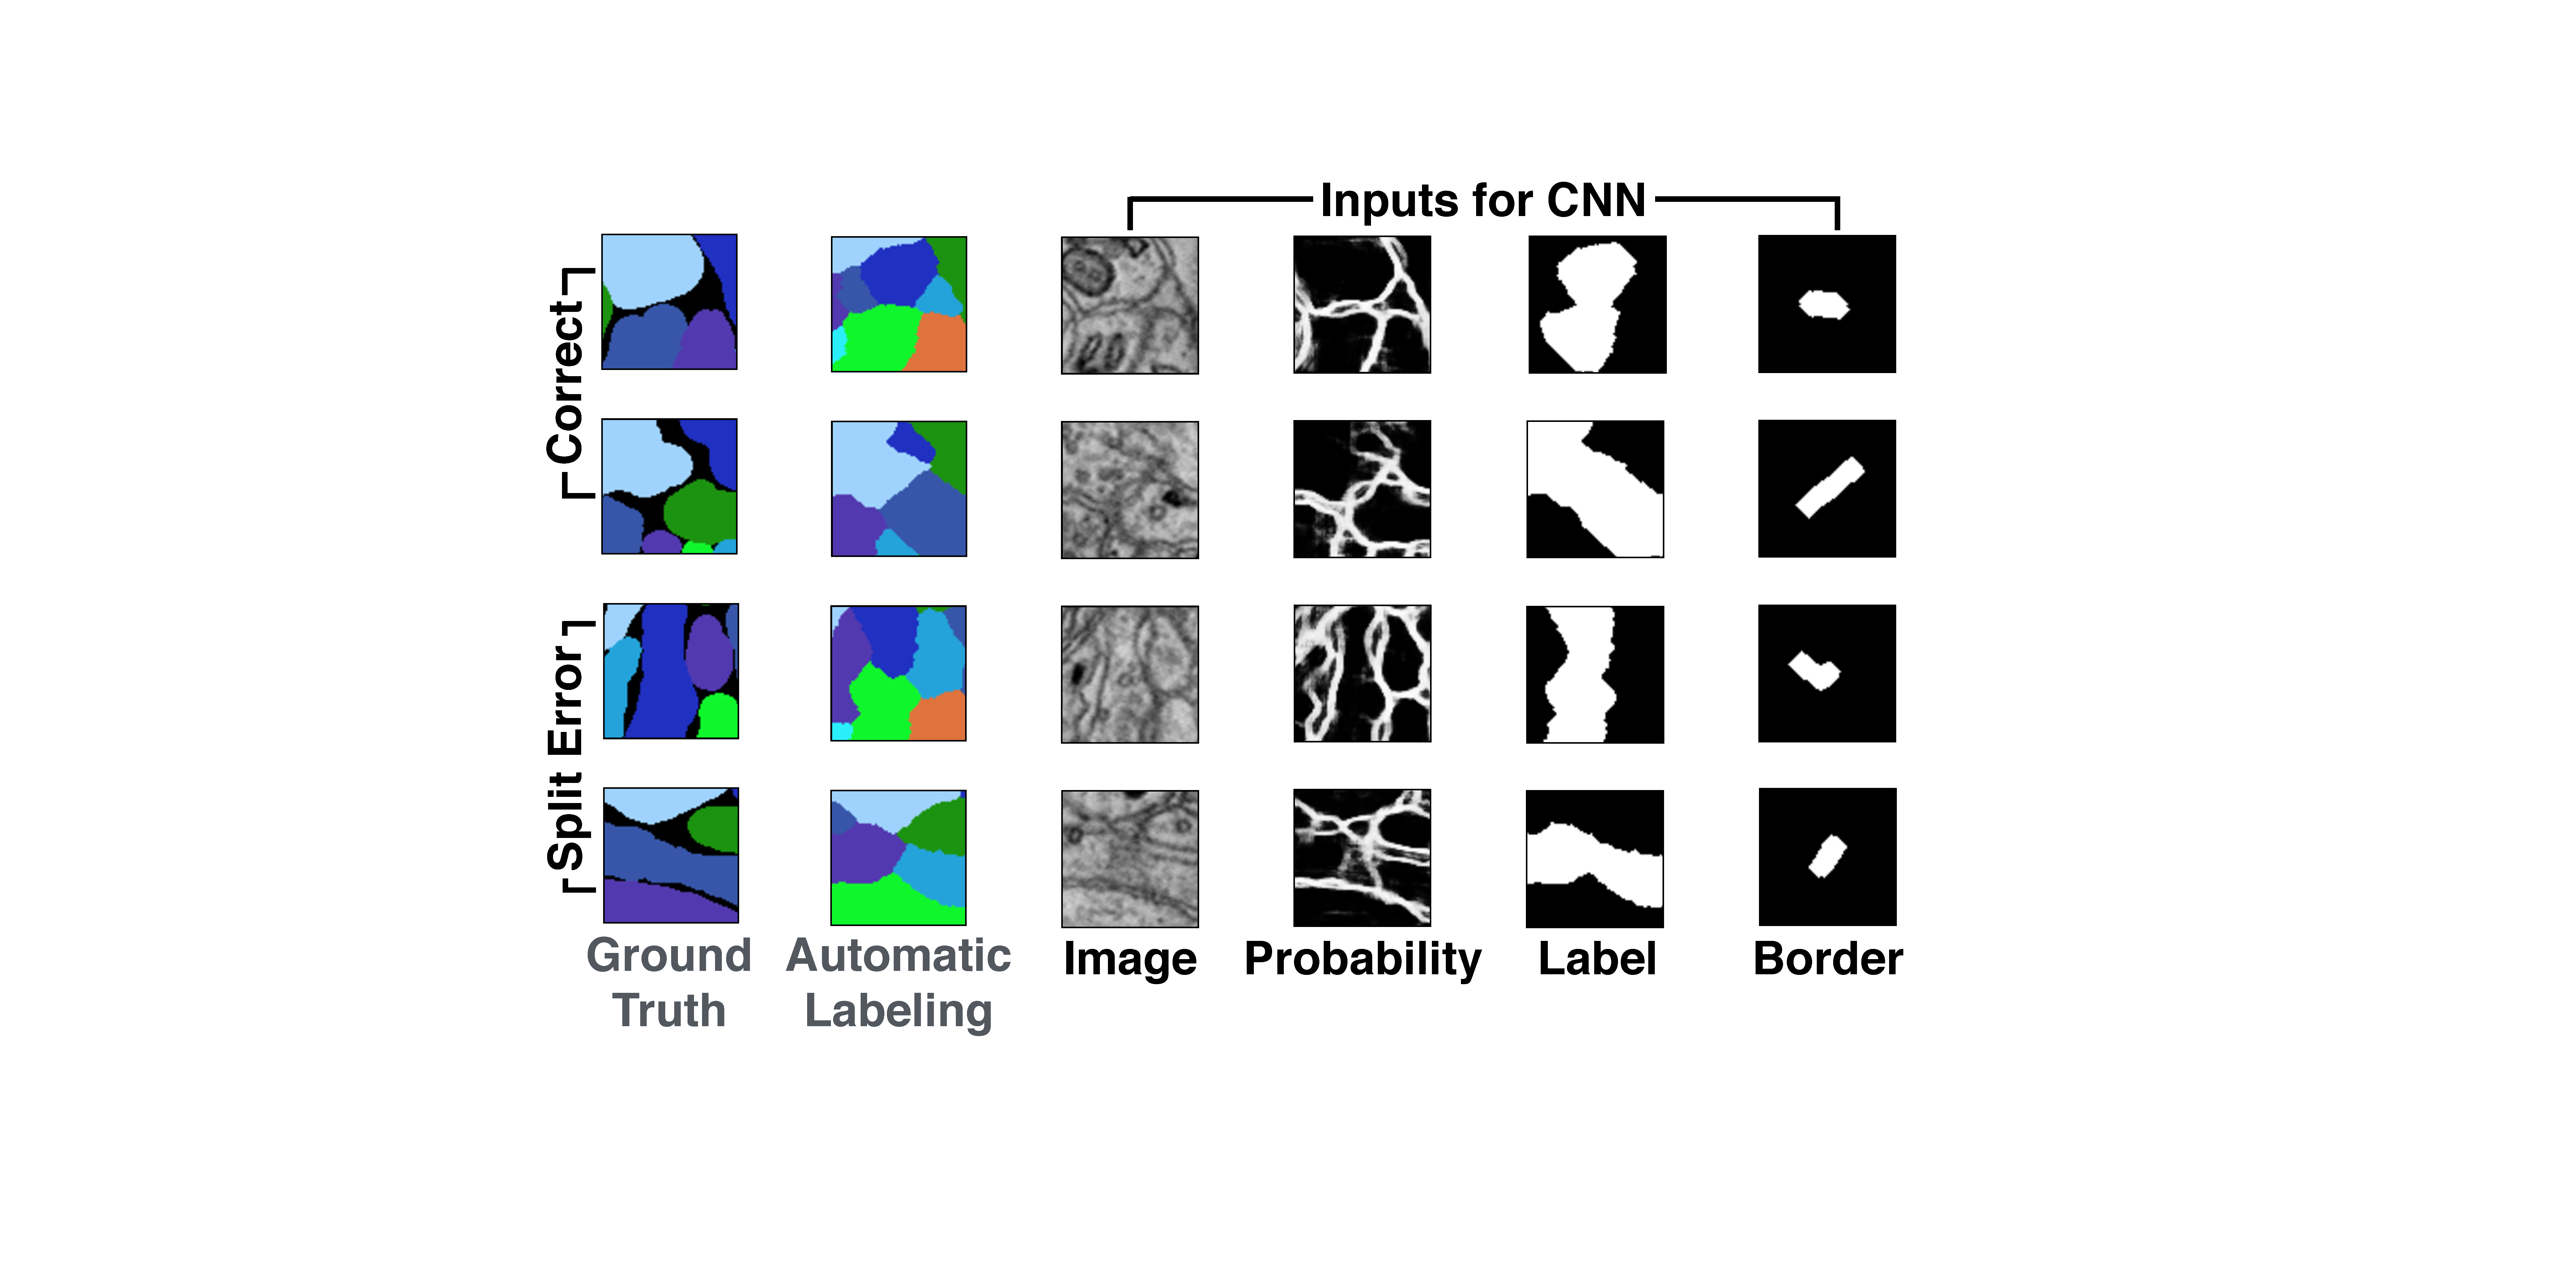
\includegraphics[width=\linewidth]{gfx/cnn_inputs.pdf}
\end{center}
 % \vspace{-4mm}
   \caption{Example inputs for learning correct splits and split errors as reflected in the segmentation relative to the ground truth. Image, membrane probabilities, merged binary labels, and a dilated border mask are combined to 4-channel input patches.}
\label{fig:cnn_inputs}
\end{figure}


\subsection{Merge Error Detection}

Identification and correction of merge errors is more challenging than finding and fixing split errors, because we must look inside segmentation regions for missing or incomplete boundaries and then propose the correct boundary. However, we can reuse the same trained CNN for this task. Similar to guided volume editing by Karimov~\etal~\cite{karimov_guided_volume_editing} we generate potential borders within a segment. For each segmentation label, we dilate the label by 20 pixel and generate 50 potential boundaries through the region by randomly placing watershed seed points at opposite sides of the label boundary. For watershed, we use the inverted gray scale EM image as features. This yields 50 candidate splits. 

Dilation of the segment prior to watershed is motivated by our observation that the generated split likely attaches to the real membrane boundary. These boundaries are then individually rated using our split error classifier. For this, we invert the probability score such that a correct split (previously encoded as $p=0$) is most likely a candidate for a merge error (now encoded as $p=1$). In other words, if a generated boundary is ranked as correct, it probably should be in the segmentation. Fig. \ref{fig:merge_error} illustrates this procedure.

\begin{figure}[h]
\begin{center}
  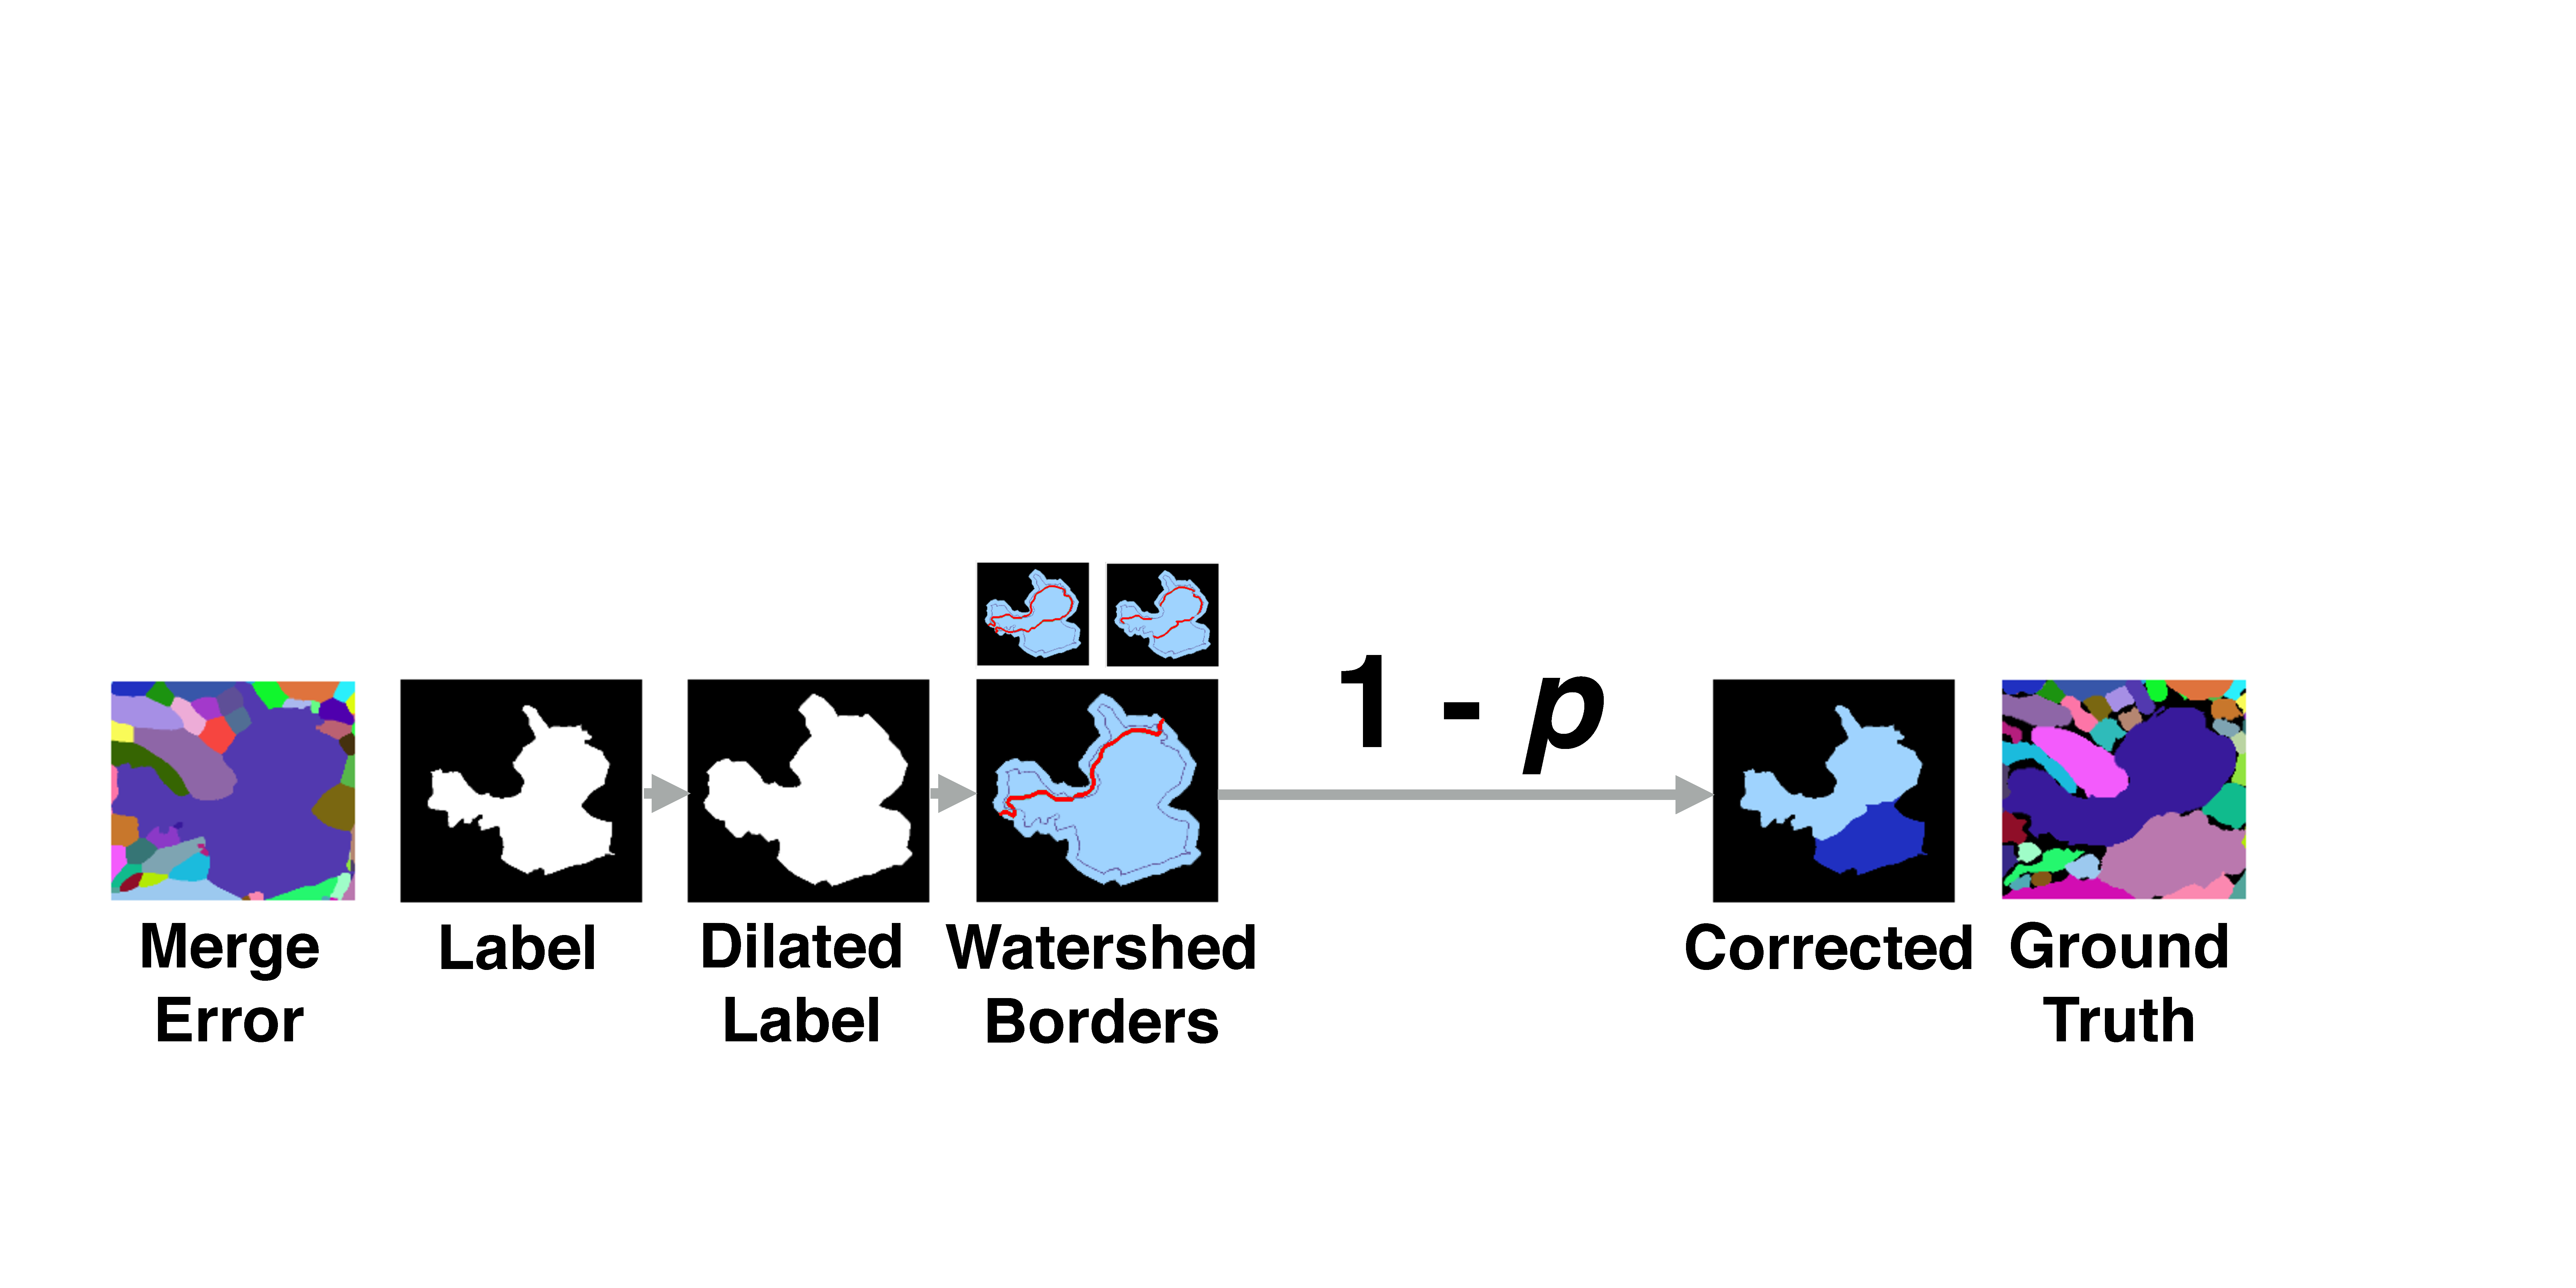
\includegraphics[width=\linewidth]{gfx/merge_error.pdf}
\end{center}
%  \vspace{-4mm}
   \caption{Merge errors are identified by generating randomly seeded watershed borders within a dilated label segment. These borders then are individually rated using the split error CNN by inverting the probability score. This way, a confident rating for a correct split most likely indicates the missing border of the merge error and can be used for correcting the labeling.}
\label{fig:merge_error}
\end{figure}

\subsection{Error Correction}

We use the proposed classifiers in combination to perform corrections of split and merge errors in automatic segmentations. For this, we first perform merge error detection for all existing segments in a dataset and store the inverted rankings $1-p$ as well as potential corrections. After that, we perform split error detection and store the ranking $p$ for all neighboring segments in the segmentation. We then sort the merge and split error rankings individually from highest to lowest. 
For error correction, we first loop through the potential merge error regions and then through the potential split error regions. During this process, each error is now subject to a yes/no decision which can be provided in different ways: 
\\~\\
\textbf{Selection oracle.} If ground data is available, the selection oracle \textit{knows} whether a possible correction improves an automatic segmentation. This is realized by simply applying the correction and comparing the outcome using a defined measure. The oracle only accepts corrections which improve the automatic segmentation - others get 
discarded. This equals perfect proofreading.
\\~\\
\textbf{Automatic selection with threshold.} The decision whether to accept or reject a potential correction is done by comparing rankings to a threshold $p_t$. If the inverted score $1-p$ of a merge error is higher than a threshold $1-p_t$, the correction is accepted. Similarly, a correction is accepted for a split error if the ranking $p$ is higher than $p_t$. Our experiments have shown that the threshold $p_t$ is the same for merge and split errors which makes sense for a balanced classifier.
\\~\\
\textbf{Forced choice setting.} A user is presented with the choices of either accepting or rejecting a correction. This way, all potential split errors are looked at. Inspecting all merge errors is not possible for users due to the sheer amount of generated borders. We therefor only present merge errors which satisfy $1-p_t$. 
\\~\\
In all cases, a decision has to be made to advance to the next possible erroneous region. If a merge error correction was accepted, the newly found boundary is added to the segmentation data. This partially updates the merge error and split error ranking in respect of the new segment. If a split error correction was accepted, two segments are merged in the segmentation data and the disappearing segment is removed from all error rankings. We then perform merge error detection on the now larger segment and update the ranking. We also update the split error rankings to include all new neighbors and re-sort. The error with the next highest ranking is now subject to the yes/no decision.

\subsection{User Interface}

Guided proofreading is integrated into an existing workflow for large connectomics data. The system is web-based and is designed with a minimalistic user interface showing three components. We show the outline of the current labeling of a cell boundary and its proposed correction on top of the EM image data. For the user, it is not possible to distinguish the current labeling and the proposed correction to avoid selection bias. We also show a solid overlay of the current and the proposed labeling. In addition, we show the image without overlays to provide an unoccluded view. User interaction is simple and involves one mouse click on either the current labeling or the correction. After interaction, the next potential error is shown. Figure \ref{fig:ui} shows the user interface.

\begin{figure}[h]
\begin{center}
  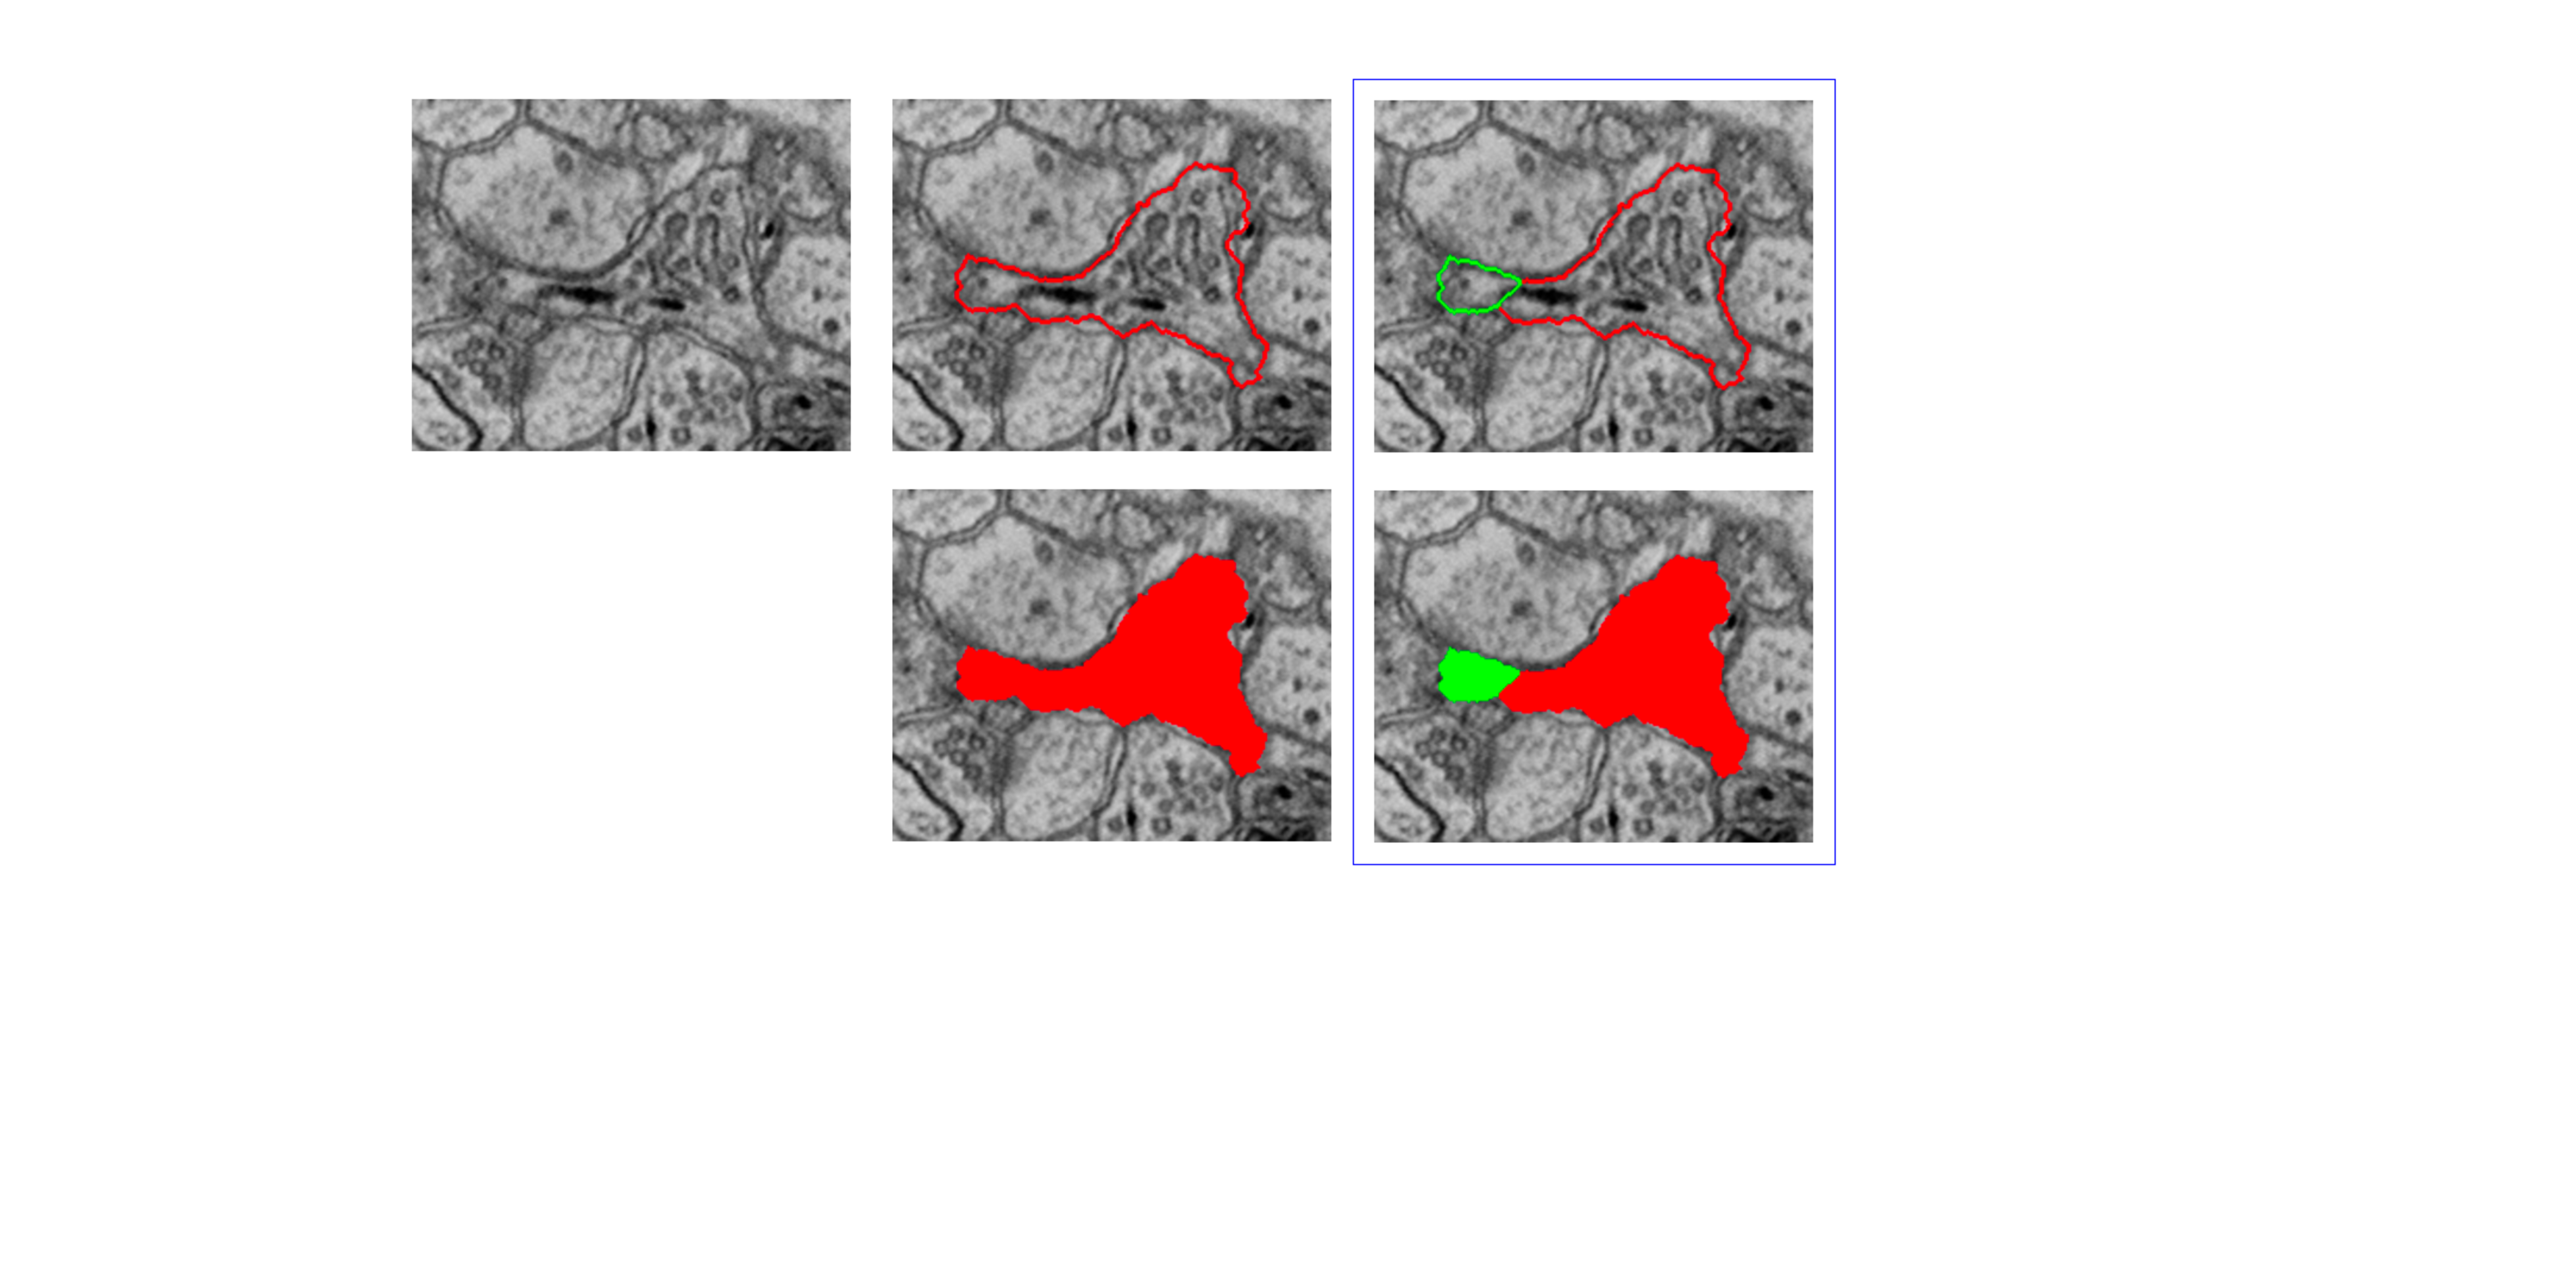
\includegraphics[width=\linewidth]{gfx/user_interface_split.pdf}
\end{center}
  \vspace{-4mm}
   \caption{Segmentation correction with the guided proofreading user interface. An image without overlays is shown on the left. A split error (right) and its correction (center) are the possible choices for the user. Hovering highlights the current selection with a yellow border and a mouse click confirms it and advances to the next potential error.}
\label{fig:ui}
\end{figure}

%
%\subsection{Active Label Suggestion}
%
%In an interactive setting, one way to present patches to the user for proofreading is to order them by the confidence probability of the GP classifier. However, in an active learning setting, where the network is retrained repeatedly on new label evidence, this approach is less likely to decrease segmentation error as, with the new labels, we are only reinforcing what the network already has a high confidence in.
%Instead, we apply active label suggestion to guide the user into labeling patches which will be more informative to retraining, and so overall decrease VI faster within the proofreading cycle of label $\rightarrow$ train $\rightarrow$ label. For each patch, we remove the softmax classification layer and look at the activation weights associated with the last dense layer. These become a high-dimensional feature vector. Then, we adapt Anon~\etal~\cite{ANON} to provide label suggestions based on features from the learned CNN, which is based on maximizing the average information gain provided by a candidate patch to label.
%A second consideration is that each patch labeled by the user provides evidence to other patches, e.g., correcting a split error redefines an entire boundary, from which multiple candidate patch labelings could have been drawn. As such, when the user labels a patch, we consider all `knock-on' effect patches as also being labeled, and feed these into the active label suggestion system similarly.
%In section \ref{sec:evaluation}, we report the difference in performance from using active label suggestion rather than confidence ordering when presenting patches to the user. These results are without retraining the network after new labelings: this should improve results, but would have to be batched to reduce computational load; hence, we leave this for future work.

 